%---------------------导言区---------------------------%
\documentclass[12pt,a4paper,UTF8]{ctexart}
\usepackage{geometry}
	\geometry{left=2.5cm,right=2.5cm,top=3.2cm,bottom=2.8cm}
\usepackage{xeCJK,amsmath,paralist,enumitem,booktabs,multirow,graphicx,subfig,setspace,listings,lastpage}
	\setlength{\parindent}{2em}
	\lstset{language=Python}
\usepackage{fancyhdr}
	\pagestyle{fancy}
	\rhead{实验 B13 利用超声光栅测量液体中的声速}
	\lhead{基础物理实验\uppercase\expandafter{\romannumeral2}实验报告}
	\cfoot{Page \thepage/\pageref{LastPage}}  %当前页\总页数
	\rfoot{\today}
	\renewcommand{\headrulewidth}{0.4pt}
	\renewcommand{\theenumi}{(\arabic{enumi})}

%%begin-----------------参考文献-----------------------%%
\usepackage[colorlinks,linkcolor=blue,urlcolor=blue]{hyperref}
\usepackage[hyperref=true,backend=biber,bibstyle=gb7714-2015,citestyle=numeric-comp,sorting=none,backref=true]{biblatex}
\addbibresource{B13.bib}
%%end-------------------参考文献-----------------------%%
%%%%%%%%%%%%%%%%%%%%%%%%%正文开始%%%%%%%%%%%%%%%%%%%%%%%%%%

\begin{document}

%%begin-------------------标题与信息-----------------------%%

%%标题
\begin{center}
\LARGE\textbf{实验 B13 利用超声光栅测量液体中的声速}
\end{center}

%%信息
\begin{doublespacing}
	\centering
	\begin{tabular}{ll}
	 & \\
	{\CJKfontspec{Droid Sans Fallback} 实验人:黄子维 20980066} & {\CJKfontspec{Droid Sans Fallback}合作者:黄睿杰 20980062}\\
	{\CJKfontspec{Droid Sans Fallback} 实验时间:2021.10.30~星期四~上午} & {\CJKfontspec{Droid Sans Fallback} 室温:27$^{\circ}$C~相对湿度:62\%}
	\end{tabular}
\end{doublespacing}
%%end-------------------标题与信息-----------------------%%

\subsection*{【实验目的】}
	\begin{enumerate}[label=\arabic*.]
		\item 了解超声波的基本性质
		\item 学习超声光栅的工作原理
		\item 利用超声光栅测量液体中的声速
	\end{enumerate}

\subsection*{【实验仪器】}
	\begin{table}[htbp]
		\centering
		\begin{tabular}{cccp{20em}}
		\toprule
		编号    & 仪器用具名称 & 数量    & 主要参数(型号,测量范围,测量精度等) \\
		\midrule
		1     &超声光栅池 &1	& / \\
		2     &超声信号发生器 &1 &KF-WSG \\ 
		3     &分光计 &1 &KF-JJYI  \\ 
		4     &低压钠灯 &1 &KFGP20Na \\
		5     &测微目镜 &1 & / \\ 
		\bottomrule
		\end{tabular}
		\label{tab:device}
    \end{table}



\subsection*{【实验原理】}
\subsubsection*{1. 介质中的超声波}
超声波:振动频率超过 20kHz 的机械波
\paragraph*{超声在介质中的传播}~
    \newline
    \indent
    \begin{itemize}
			\item 基本量:声速,衰减系数。
			\item 在正弦变化的超声声场中,由于声压作用,介质折射率呈周期变化:
			\begin{equation}
			n(y,t)=n_0+\Delta n cos(\omega t-ky)
			\end{equation}
	\end{itemize}
\paragraph*{驻波和行波}~
    \newline
    \indent
	正弦超声平面波垂直射入液体中时,声场中的压力波被液槽侧面反射,形成与入射波同频率的一列反射波,这两列波的压强可以分别表示为:
	\begin{equation}
		\begin{cases}
			&P_i=P_{i_A}e^{i(\omega t-ky)} \\
			&P_r=P_{r_A}e^{i(\omega t+ky)}\\
		\end{cases}
	\end{equation}	
	两同频波反向传播,依叠加原理,合成声场的声压为$P=P_i+P_r$,即	
	\begin{equation}
		P=2P_icos(kye^{i\omega t})+(P_{i_A}-P_{r_A})e^{i(\omega t-ky)}
	\end{equation}
	由上式,合成声场由两部分组成,第一项代表驻波场,第二项表示在Y方向进行的平面波场,其振幅为原先两列波振幅之差。
	
	若实验中弹性的平面波得到完全反射,则上式右边第二项可以略去。
	这样合成的超声场就是一个纯粹的驻波场。
	
	在该驻波场的作用下,介质密度和折射率的分布也与驻波场的变化相一致。
	声压形成的光密处为波节,光疏处为波腹。如图\ref{fig:illus-1}所示。
	\begin{figure}[htbp]
		\centering
		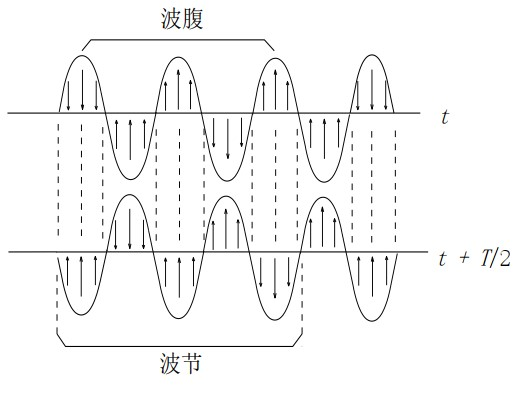
\includegraphics{attachments//illus-1.jpg}
		\caption{超声驻波的运动}
		\label{fig:illus-1}
	\end{figure}
	
	需要注意的是,从密度或折射率变化的相对位置看,如图\ref{fig:illus-2a},在(t+T)/2时的波形相对于t时刻的波形来说,好像光栅相对向右移动了半个波长。
	而在任何时刻相距为λ的两点处,液体的密度是相同的。
	由于光向折射率大的方面弯曲,所以波节处交迭地每隔半个周期呈现一次汇聚强光。
	这种周期性的变化人眼看不出来,实验观察到的超声场的图像,是相对的长时间的平均效应。
	图\ref{fig:illus-2b}就是在声压作用下,超声场中介质疏密的瞬时分布。
	行波的疏密波会向前传播。
	\begin{figure}[htbp]
		\centering
		\subfloat[超声驻波的疏密分布]{\label{fig:illus-2a}
		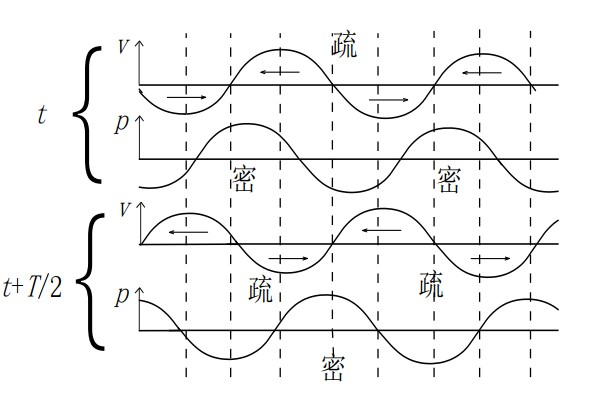
\includegraphics[width=0.4\textwidth]{attachments/illus-2a.jpg}
		}%
		\subfloat[超声驻波速度和声压的分布]{\label{fig:illus-2b}
		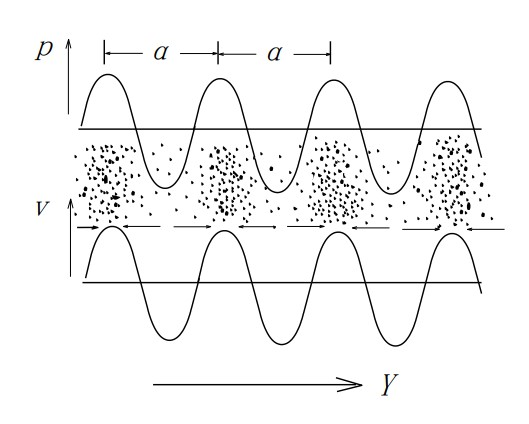
\includegraphics[width=0.4\textwidth]{attachments/illus-2b.jpg}
		}%
		\caption{超声驻波}
	\end{figure}

\subsubsection*{2.超声光栅}
	\paragraph{原理}~
	\newline
	\indent
	平面超声波在液体介质中传播时,其声压使液体产生疏密交叠的变化,从而液体的折射率也相应出现周期性变化,形成超声光栅(如图\ref{fig:illus-3})。
	当光沿垂直方向透射过超声场后,将会产生折射和衍射。
	\begin{figure}[htbp]
		\centering
		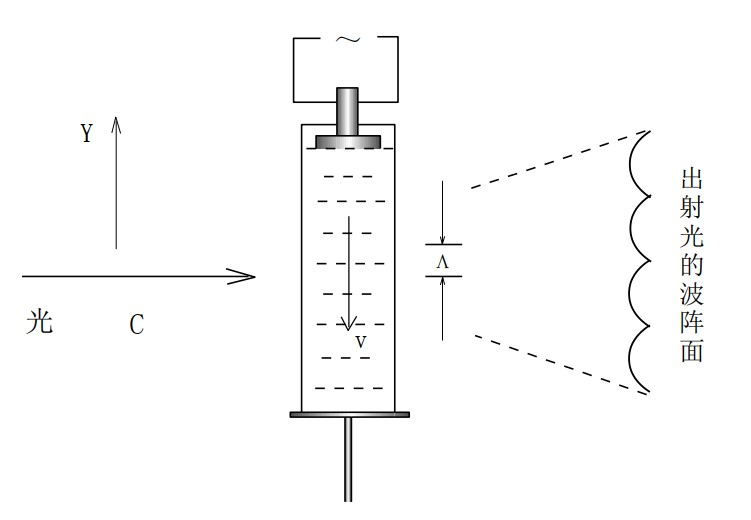
\includegraphics[width=0.6\textwidth]{attachments//illus-3.jpg}
		\caption{超声光栅示意图}
		\label{fig:illus-3}
	\end{figure}

	因光速远大于声速,光线很快的通过了超声场,从而折射率不同层次所形成的超声光栅可认为不动。因此折射率空间分布可以视为:
	\begin{equation}
	N=N_0+\varDelta N cos(ky)
	\end{equation}	

	\paragraph{超声衍射以及声速测量}~
	\newline
	\indent
	超声光栅对光的衍射可表示为:
	\begin{equation}\label{eq:1}
		\varLambda sin \theta_K = \pm K\lambda
	\end{equation}
	式\ref{eq:1}中$\varLambda $和$\lambda$分别为超声波和光波的波长,$\theta_K $为K级衍射角。

	若测出$\theta_K$,且$\lambda$已知,则可计算出超声波的波长$\varLambda$ ,若已知超声波的频率$f$,则可求出超声波在该液体中的传播速度:
	\begin{equation}\label{eq:2}
		u=\varLambda f
	\end{equation}

\subsubsection*{3.超声场的观测}
	光路如图\ref{fig:illus-4}所示,将超声光栅液体池$AB$放在分光计的载物台上,其中$B$为超声源。则可在望远镜中观察到系列平行条纹。
	利用分光计可以测量出条纹的衍射角,进而测出超声波的波长$\Lambda $,并根据超声波的频率$f$,利用式\ref{eq:2}计算出超声波在液体中传播的速度。
	\begin{figure}[htbp]
		\centering
		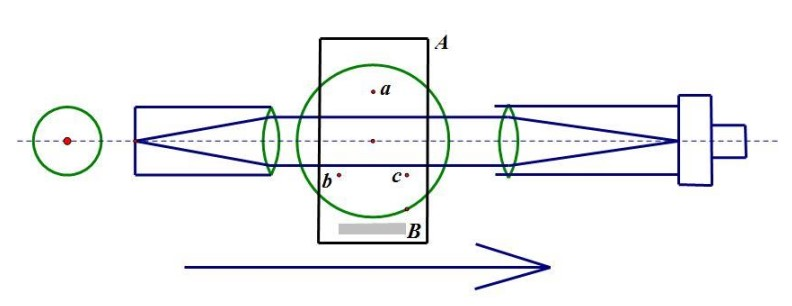
\includegraphics[width=0.5\textwidth]{attachments/illus-4.jpg}
		\caption{中心暗条纹}
		\label{fig:illus-4}
	\end{figure}

	为提高测量精度,可将望远镜目镜换成测微目镜进行观察。
	条纹像落在测微目镜的焦平面上,条纹清晰。用测微目镜测出条纹间距x,可将条纹的衍射角表示为:
	\begin{equation}\label{eq:3}
		tan \theta_K\approx sin\theta_K=\frac{x}{F}
	\end{equation}
	其中F为测微目镜的焦距。根据式\ref{eq:1}和式\ref{eq:3}可得
	\begin{equation}
		\frac{K\lambda}{\varLambda }=\frac{x}{F}
	\end{equation}
	则
	\begin{equation}
		\frac{x}{fF}=\frac{\lambda}{f\varLambda}=\frac{\lambda}{u}
	\end{equation}
	其中u是要测的声速,f为超声波的频率,则被测液体中的声速可表示为
	\begin{equation}\label{eq:4}
		u=\frac{\lambda F f}{x}
	\end{equation}
 
\subsection*{【实验装置】}
实验装置如图\ref{fig:5}所示。若不采用测微目镜,只是使用分光计测量超声光栅的衍射角,则可不安装测微目镜(8),采用望远镜目镜和显示器代替。
\begin{figure}[htbp]
	\centering
	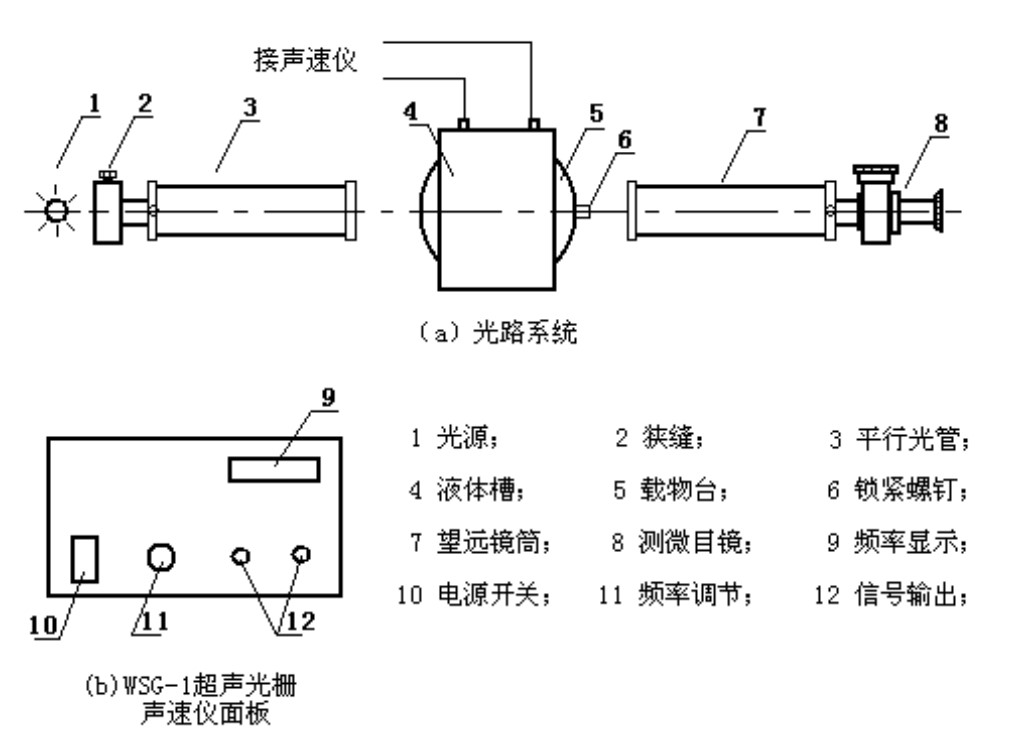
\includegraphics[width=0.8\textwidth]{attachments//illus-5.jpg}
	\caption{超声光栅实验装置图}
	\label{fig:5}
\end{figure}

    \paragraph{注意事项}~
    \newline
    \indent
    \begin{enumerate}[label=\arabic*.]
		\item 实验结束,超声池中的水应尽快清理,不应长时间浸泡在液体槽内。
		\item 超声仪的频率易受外界环境的影响,只要外界变化使其导线电容分布发生变化,就有可能会对输出频率产生影响,应尽量避免震动及触碰导线。
		\item 若该实验原配的超声信号发生器工作不稳定,可采用函数信号发生器替代,但采用原厂设备可观察到3级衍射谱,采用替代设备只能观察到2级衍射谱。同时函数信号发生器的输出信号峰峰值不要超过18V。
	\end{enumerate}


\subsection*{【实验内容及步骤】}

\subsubsection*{1.实验装置调节}
    \begin{enumerate}[label=\arabic*.]
		\item 调节分光计到正常测量状态,平行光管与望远镜准直同轴。
		\item 在超声光栅盒中加入适量的水,并固定在分光计载物台上。转动游标盘使光栅盒正面玻璃反射的绿色十字像的垂直线和水平线与十字叉丝的垂直线和水平线重合。并连
		接超声盒电路。
		\item 打开光源,在望远镜中可看到一条竖直亮条纹。微调望远镜和狭缝宽度使条纹清晰,并使条纹与望远镜垂直叉丝重合。记录角度$\theta_0$.
		\item 打开超声源开关,微调超声波频率,使视野中出现尽可能多的衍射条纹且条纹清晰。
	\end{enumerate}

\subsubsection*{2.采用衍射角法测量声速}

直接采用分光计的望远镜目镜,测量不同条纹的衍射角,根据式(5)和式(6)计算液体中超声波的波长$\varLambda$ 计算液体中声速u.
\subsubsection*{3.采用测微目镜测量声速}

采用测微目镜替换望远镜目镜。在观察到清晰条纹后,转动测微目镜上的鼓轮,测量每条条纹的位置,用逐差法求出条纹间距x,利用式(10)计算液体中声速u.
请自列表格记录数据和计算,并分析结果的不确定度。

\subsection*{【数据处理及分析】}
	\subsubsection*{1. 采用衍射角法测量纯水声速}
		\paragraph{实验参数} 钠黄光波长$\lambda = 589.3 nm$,超声频率$f = 10.64 MHz$
		\paragraph{实验数据}~
		\newline
		\indent
		利用分光计望远镜目镜,测量超声光栅不同级次条纹的衍射角,原始数据如表\ref{tab:1}。表格中角度均以弧度制表示,$k$为衍级次,$\theta_1$和$\theta_2$分别为k级次两游标读数,$\theta$为消除偏心差后角度值。
		\begin{table}[htbp]
			\centering
			\begin{tabular}{|l|l|l|l|}
			\hline
				k & $\theta_1$ & $\theta_2$ & $\theta$ \\ \hline
				-3 & 1.735148 & 4.879068 & 1.736312 \\ \hline
				-2 & 1.730785 & 4.874414 & 1.731803 \\ \hline
				-1 & 1.726131 & 4.870050 & 1.727294 \\ \hline
				0 & 1.721767 & 4.865105 & 1.722640 \\ \hline
				1 & 1.717986 & 4.861615 & 1.719004 \\ \hline
				2 & 1.713622 & 4.856960 & 1.714495 \\ \hline
				3 & 1.708968 & 4.852597 & 1.709986 \\ \hline
			\end{tabular}
			\caption{衍射角法实验原始数据}
			\label{tab:1}
		\end{table}

		计算k级条纹角度值与零级条纹角度值之差,得到各级条纹角位置,并计算正弦值。如表\ref{tab:2}。
		\begin{table}[htbp]
			\centering
			\begin{tabular}{|l|l|l|}
			\hline
				k & $\theta_k$ & $sin\theta_k$ \\ \hline
				-3 & -0.013672 & -0.013671 \\ \hline
				-2 & -0.009163 & -0.009163 \\ \hline
				-1 & -0.004654 & -0.004654 \\ \hline
				0 & -0.000000 & -0.000000 \\ \hline
				1 & 0.003636 & 0.003636 \\ \hline
				2 & 0.008145 & 0.008145 \\ \hline
				3 & 0.012654 & 0.012653 \\ \hline
			\end{tabular}
			\caption{衍射条纹角位置}
			\label{tab:2}
		\end{table}
		
		\paragraph{拟合$k-sin\theta_k$曲线计算声速值}~
		\newline
		\indent
		拟合$k-sin\theta_k$曲线,结果如图\ref{fig:1}。直线斜率为229.59。
		\begin{figure}[htbp]
			\centering
			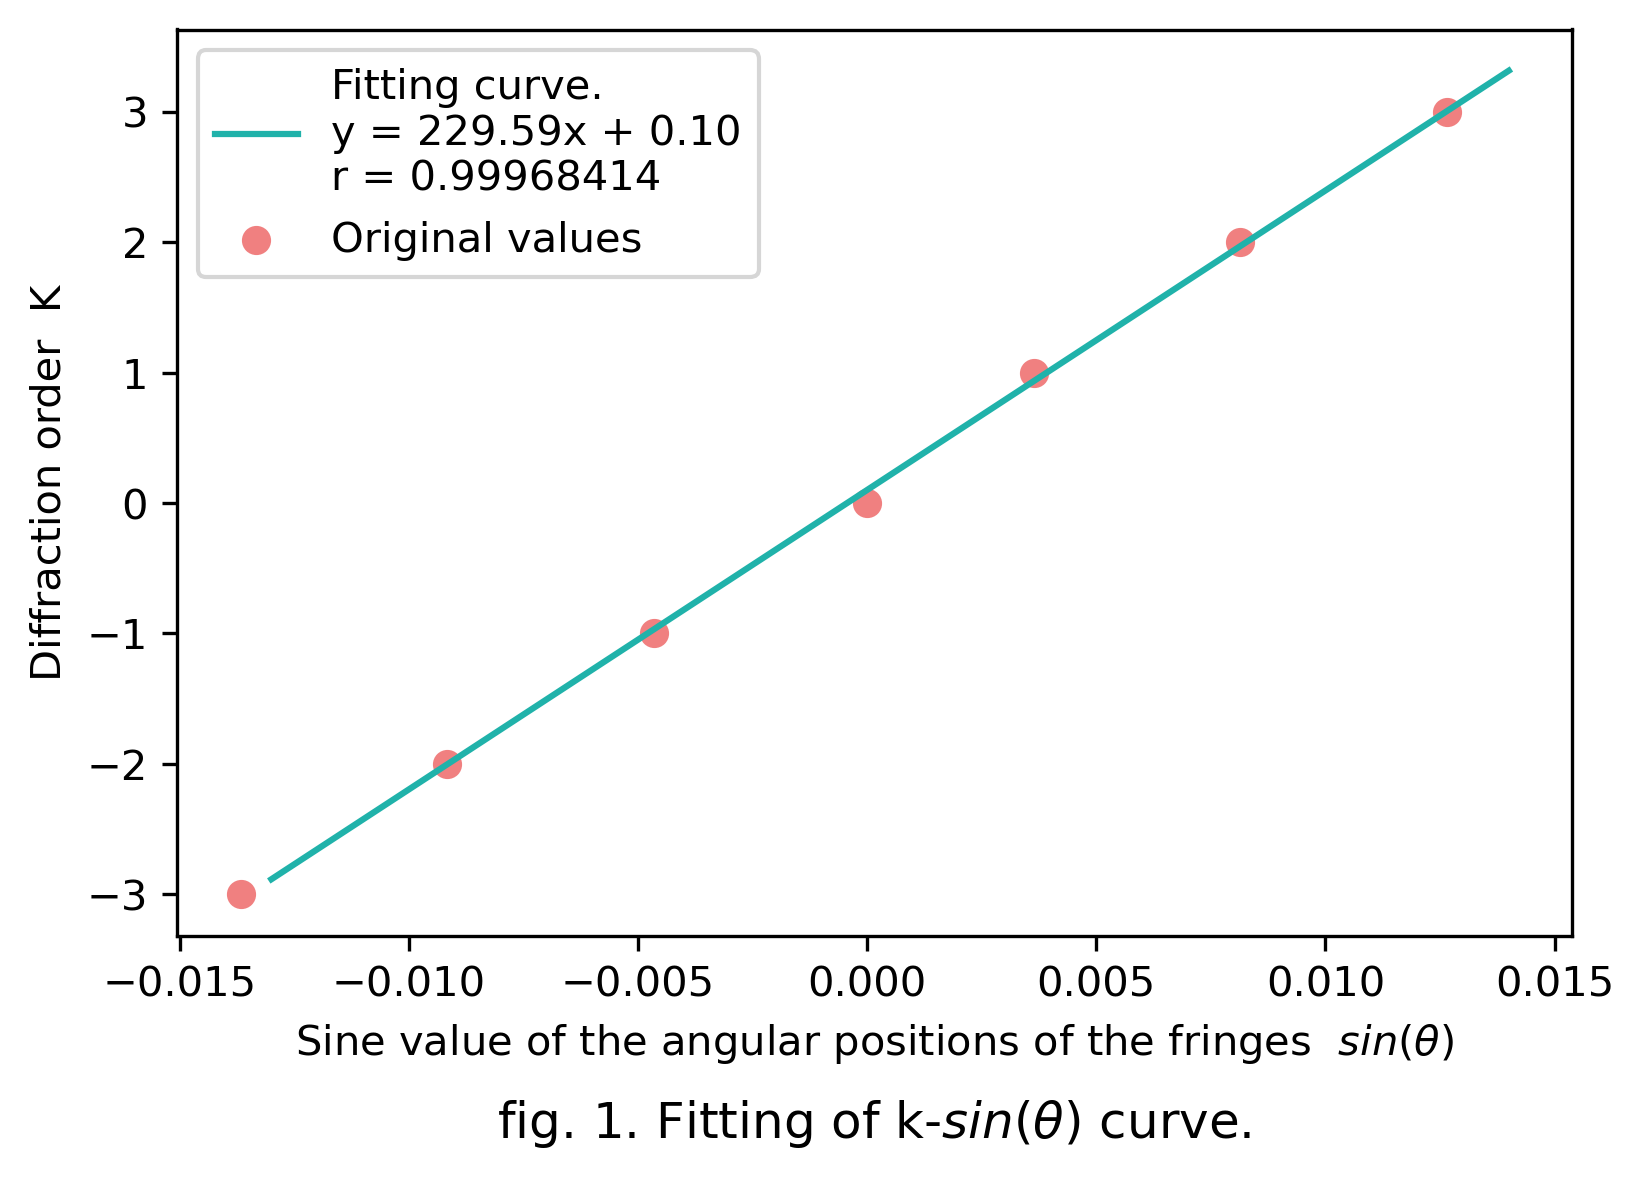
\includegraphics[width=0.7\textwidth]{attachments/fig.1.png}
			\caption{拟合$k-sin\theta_k$曲线}
			\label{fig:1}
		\end{figure}
		
		由式\ref{eq:1}和式\ref{eq:2}得声速计算公式
		\begin{equation}\label{eq:5}
			u = f\lambda\frac{k}{sin(\theta_k)}
		\end{equation}
		
		代入直线斜率和实验参数,计算得
		$$
		u = 1439.56 m/s
		$$

		
	\subsubsection*{2. 采用测微目镜测量声速}
		\paragraph{实验参数} 钠黄光波长$\lambda = 589.3 nm$,超声频率$f = 10.64 MHz$,测微目镜焦距$F = 170mm$
		\paragraph{实验数据}~
		\newline
		\indent
		利用测微目镜,测量超声光栅不同级次条纹的位置,原始数据如表\ref{tab:3}。$k$为衍射级次,$x$为条纹位置
		\begin{table}[htbp]
			\centering
			\begin{tabular}{|l|l|}
			\hline
				k & x/mm \\ \hline
				-3 & 2.895 \\ \hline
				-2 & 3.600 \\ \hline
				-1 & 4.315 \\ \hline
				0 & 5.000 \\ \hline
				1 & 5.735 \\ \hline
				2 & 6.410 \\ \hline
				3 & 7.105 \\ \hline
			\end{tabular}
			\caption{测微目镜测量原始数据}
			\label{tab:3}
		\end{table}

		计算k级条纹位置与零级条纹位置之差,得到各级条纹位置,如表\ref{tab:4}。
		\begin{table}[htbp]
			\centering
			\begin{tabular}{|l|l|}
			\hline
				k & x/m \\ \hline
				-3 & -0.002105 \\ \hline
				-2 & -0.001400 \\ \hline
				-1 & -0.000685 \\ \hline
				0 & 0.000000 \\ \hline
				1 & 0.000735 \\ \hline
				2 & 0.001410 \\ \hline
				3 & 0.002105 \\ \hline
			\end{tabular}
			\caption{衍射条纹角位置}
			\label{tab:4}
		\end{table}
		
		\paragraph{拟合$k-x$曲线计算声速值}~
		\newline
		\indent
		拟合$k-x$曲线,结果如图\ref{fig:2}。直线斜率为1423.39。
		\begin{figure}[htbp]
			\centering
			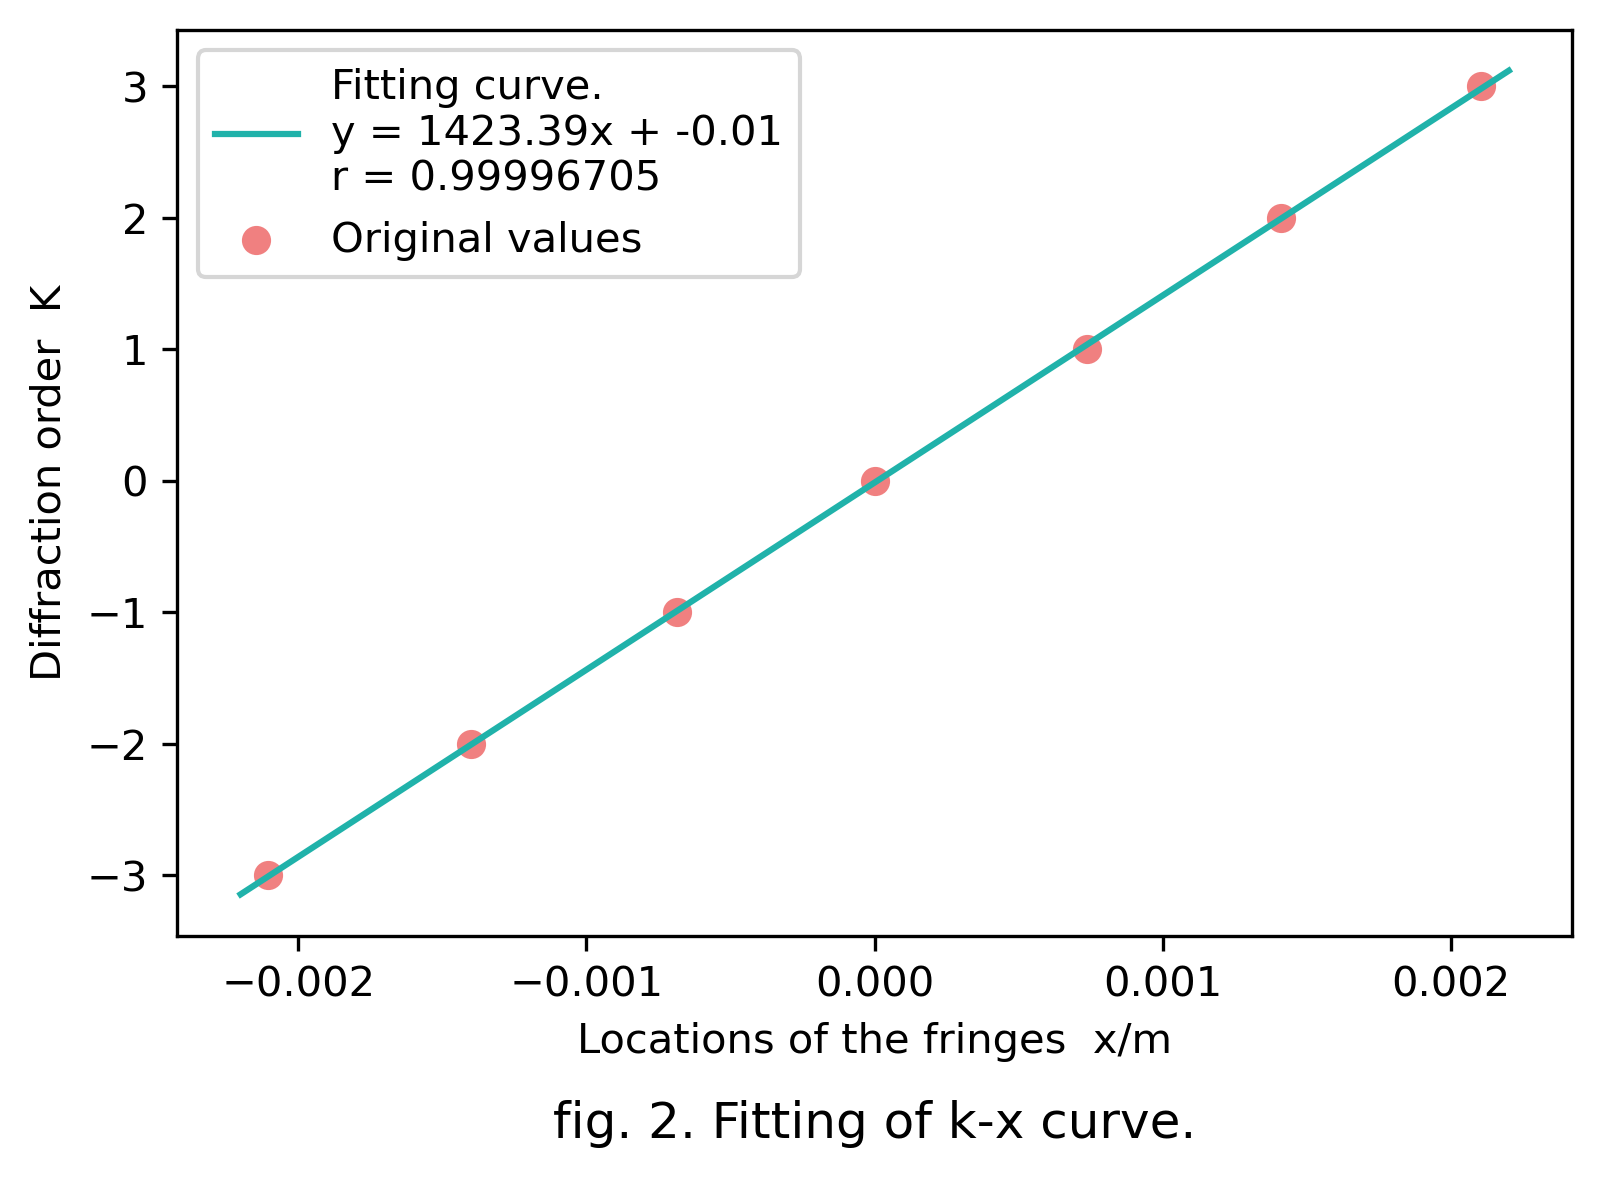
\includegraphics[width=0.7\textwidth]{attachments/fig.2.png}
			\caption{拟合$k-x$曲线}
			\label{fig:2}
		\end{figure}
		
		由声速计算公式\ref{eq:4},式中$x$为条纹角间距,即为上述拟合直线斜率的倒数。代入直线斜率和实验参数,计算得
		$$
		u = 1517.23 m/s
		$$
\subsection*{【实验结果分析】}
实验温度为$27^oC$,由纯水声速计算公式$u = 1404.3 + 4.7T - 0.04T^2$\cite{LUBBERS19981065}得声速理论值$u = 1502.04 m/s$。

衍射角法测量值为$u = 1439.56 m/s$,相对误差为$4.15\%$,拟合相关系数为$0.99968$。

测微目镜法测量值为$u = 1517.13 m/s$,相对误差为$1.01\%$,拟合相关系数为$0.99997$。

可见测微目镜法测量声速能获得更高的准确度。
这是因为衍射角法测量需要手动转动分光计,转动角度无法精确控制,测量有较大误差。而使用测微目镜法测量只需调节转动螺旋测微头,调节更加方便且精细,读数精度更高,测量误差较小。
%%end--------------------引用------------------------%%
\printbibliography[title=参考文献] %title:默认是英文的reference,用这个选参数改成中文
%%end--------------------引用------------------------%%

\newpage
\subsection*{【思考题】}
	\subsubsection*{1. 由驻波理论知道,相邻波腹间的距离和相邻波节间的距离都等于半波长,为什么超声光栅的光栅常数等于超声波的波长呢?}
		\begin{enumerate}[label=\arabic*.]
			\item 超声波驻波为纵向振动驻波。
			\item 考虑某时刻纵驻波的某一波节,该波节两侧的质点都涌向这个波节的中心,使该节点附近的成为质点密集区,而相邻的波节处为质点稀疏区。
			\item 半个周期后,这个节点附近的质点向两边散开,该波节变为稀疏区,相邻的波节处变为密集区。稀疏处液体折射率小,而压缩处液体折射率增大,光通过后将形成衍射条纹。
			\item 但事实上,这种周期性变化在人眼看来无法分辨的,观测到的干涉图样是长时间平均效应。
			\item 实际上,在任意时刻距离等于波长$\lambda$的两点,液体的密度相同,折射率也相同。
			\item 因此超声光栅的光栅常数等于超声波的波长。
		\end{enumerate}
	\subsubsection*{2. 比较超声光栅与平面光栅的异同。}
		同:
		\begin{enumerate}[label=\arabic*.]
			\item 具有类似的光学性质,都能使光发生衍射
			\item 衍射图样主极大满足类似的光栅方程
			\item 都会发生缺级
		\end{enumerate}
		
		异:
		\begin{enumerate}[label=\arabic*.]
			\item 超声光栅是动态光栅,衍射图样是时间平均结果;而平面光栅是静态光栅,没有频移现象。
			\item 衍射图样衍射条纹强度分布不同
			\item 缺级发生的原理不同
		\end{enumerate}
	\subsubsection*{3. 有的教材中,超声光栅实验的超声波频率为200kHz,请问此时能用光栅的原理解释实验结果吗?为什么?}
		答:由式\ref{eq:5},对于同一声速下同一光波长的同一衍射级而言,超声频率越低,则衍射角越小,即衍射条纹更密。当超声频率过低时,由瑞利判据,零级衍射条纹和一级衍射条纹无法分辨,因此无法进行测量,因此不能用光栅的原理解释实验结果。
\subsection*{【项目源码】}
\href{https://github.com/Jeg-Vet/SYSU-PHY-EXP/tree/main/B13-Ultrasonic_grating}{SYSU-PHY-EXP/B13 Ultrasonic grating @Jeg-Vet(github.com)}

\end{document}
